\lhead{\emph{Design}}
\chapter{Design}
\label{sec:design}
In this chapter the design of the system is described. Although we have decided from the beginning to design a system based on head gestures and audio modalities, we will still discuss how alternative modalities based on existing systems and related research from chapter \ref{sec:relatedwork} would fit in a biking scenario. This will give a better insight of the importance of modality choice - the benefits and tradeoffs - when designing systems for interaction in-motion. Also the related systems could contribute to the design of specific features for our final system. This is part of the design rationale and covers the first part of this chapter. In the second part the final system design is presented.


\section{Design Rationale}
% Intro
Before choosing a design for a system different factors needs to be considered e.g. the reasons behind the design decisions and the justification for it, other design alternatives considerations and the tradeoffs when choosing a design over another and the argumentation that lead to the design.

% Ubicomp challenges
When designing for ubicomp new aspects needs to be taken into consideration which increase the complexity of the system e.g. different devices, mobile users and changing environment and context \cite{barfield_fundamentals_2000}. Also we note that we are not only designing user interfaces but also the interactions between a user and the system through artifacts embedded in the environment \cite{beaudouin-lafon_designing_2004}. Furthermore it should be taken into account whether the interaction happens while the user is in motion as this introduces even more complexity as decribed earlier in section \ref{sec:interactioninmotion}.

In this project we have defined the following requirements of the system: A user should navigate a music player while biking. In other words we have a user interacting with artifacts, in order to explore and select music tracks, while biking in a traffic environment implying user awareness of road conditions, cars, other bikers, etc.

As a consequence of these requirements, we will in the next sections discuss the constraints derived from a scenario like that and how modality combinations could fit in the design of such a system. This will result in a discussion on related systems, that uses the audio modality as interaction form. Last we will delve into specific related audio interfaces and look at different auditory menu designs.

\subsection{Biking scenario constraints}
% intro, physical and mental constraints
Several constraints emerge from a humans capabilities to interact with a system while biking, both physically and mentally. Seen from a physical perspective the person riding the bike needs to have both hands on the handlebars in order to dodge any sudden obstructions e.g. an inattentive car. For the same reasons, and more importantly, the persons eyes needs to focus on the road. The latter is of more importance from the fact that people can not easily divide their visual attention between tasks \cite{brewster_overcoming_2002} but two hands can work independently from each other, dedicating one for steering and one for the interface. This does not mean that one hand can steer a bike perfectly - this is subjective, and we must assume that both hands for steering is preferable. Lastly biking requires the legs/feet on the pedals to move forward. From a mental perspective biking is heavily depending on the users attention or perceptual load first of all to navigate the road but more importantly to keep the ability to react to traffical events. This perceptual load is complemented by the cognitive load which can increase in a very busy traffical biking scenarios and depends on the users ability to handle such scenarios.

From a system perspective a biking scenario also implies constraints. First of all interaction with the system should should be considered e.g. should it be provided through a wearable device or some kind of installable hardware that could be attached to the bike. The system also needs to optimize handling of unintentional interaction during biking e.g. motion gestures when riding a bumpy road. Secondly and most important the system needs to aim for minimizing the workload required by the user - every added feature should be considered i.e. every interaction task should be considering conducted while biking. Also the content presented to the user should be considered in terms of the interaction modality being used e.g. in a visual music player interface artist/track information and a lot of navigation possibilities might be good but if the same information and functionality were to provided via audio this would cause a non-linear effect (as described in section \ref{sec:interactioninmotion}) and add too much complexity to the system.

\subsection{Modalities reasoning}

% HMD, Gaze tracking
\textbf{Visual challenges}

A headmounted visual display like Google Glass would give total hands-freeness when biking but as mentioned in \ref{sec:interactioninmotion} such displays can be hard and obtrusive to use in bright daylight. Also such interface still would require the visual attention from the user \cite{geelhoed_safety_2000}, although the user would not have to change head direction while biking (like when looking down on a traditional stop-to-interact interface). Same arguments follows with a gaze tracking solution. Also such a solution could require some kind of installation on the bike e.g. a camera attached to the handlebars for tracking the eye. Mobile solutions exists \cite{mardanbegi_eye-based_2012} but this will still imply the user to look at the device, and probably hold the device i.e. occupying one hand, while interacting. However the benefit with using visual displays like the headmounted displays in our scenario is, that it's possible to keep the rich visual experience of exploring music tracks before selecting them - information could be linearly translated from the stop-to-interact music player interfaces. It can be argued though, that the experience is not as rich when biking in a traffic environment where attention is divided.

Studies on multimodal interaction \cite{zhao_shared_2013} have shown that when humans needs to attend a physical visual task and a virtual task at the same time (dual task situation) - they found it significantly distractive to attend to the virtual task in a visual way. Instead audio has shown to be less distractive. The biking while interacting scenario can easily be translated into such a dual task where the physical task is to attend to the road and traffic and virtual task is to explore and select music tracks. Inspired from this and from other studies showing that audio can improve usability with mobile devices in eyes-free mobile conditions \cite{brewster_multimodaleyes-freeinteraction_2003}, systems designs that uses audio modalities should be considered instead.

% Audio interfaces/related systems
\textbf{Audio only}

Using audio both as input and output modality is implemented in voice recognition system like the Google Search voice command system for Android or Siri on iOS mentioned in section \ref{sec:alternativemusicuis}. A good thing about this system is that the hardware requirements are minimal - it would work on all devices supporting Android and with all kinds of headsets. From a physical and workload demanding perspective this could work in a biking scenario e.g. a user would have to pick out the phone (maybe from the pocket) and then place it near the mouth and give the command. The visual attention would still be on the traffical surroundings although picking out the phone could need some attention. By using a headset controller with a mic this possible "hand attention problem" could be avoided. This interface however have some challenges \cite{sawhney_nomadic_2000} especially in noisy environments, where voice commands can be hard to recognize by the system, making it tedious and frustrating for the user to keep repeating the command. This frustration and also that the user is doing a physical activity like biking (increasing heart rate), can change the voice and affect the systems recognition abilities. At the same time these commands are limited i.e. navigation is limited. Too many commands would add heavy complexity to the system e.g. imagine a stop-to-interact music player interface like Spotify to translate just 10 of their navigation features to a voice command system. This will create a non-linear effect i.e. the user will have a hard time just remembering the commands and could get lost quickly in the navigation.

\textbf{Touch-based and audio}

Touch and audio based interfaces also suffers from limited navigation controls. Todays headset music controllers however fits well in a biking scenario. Although using one hand while biking to navigate the interface, the time it takes to push a button is short i.e. reducing the time where the bike is controlled with one hand. This short navigation maneuver is also due to the limited possible interface controls. Similar to these head controllers are the touch based interfaces that uses touch screens \cite{pielot_pocketmenu:_2012, pirhonen_gestural_2002} - controlled from the pocket. These interfaces however uses more advanced output modalities e.g. audio/tactile simultanous modalities (PocketMenu) and spatial audio feedback, which potentially could be used for richer exploration of menu items but also possibly increase complexity i.e. making it a harder cognitive task. Considering these advanced output modalities spatial audio has shown to be able to present complex information \cite{bronkhorst_cocktail_2000, gaver_sonicfinder:_1989} while keeping the human cognitive load down \cite{vazquez-alvarez_eyes-free_2011} and in combination with gesture input modalities, it was used effectively when navigating an interface in eyes-free mobile conditions. 

\textbf{Motion gestures and audio}

Considering combining spatial audio output with a motion gesture input modality, possible available human body parts when biking could be hands (implies biking with one hand) or the head. Although feet as a modality input were evaluated in a running scenario with good results \cite{smus_running_2010}, it would be awkward when biking would require both feet on the pedals to keep moving. Kajastilas free-hand gestures \cite{kajastila_interaction_2013} would imply the same hand interaction challenges discussed above but also a camera installed on the bike to detect the movements. Sensors could be used instead but would require some artefact installed on the hand. Instead it might be more appropriate to install sensors into a headset and use head movements as input modality like \cite{park_gaze-directed_2011, brewster_multimodaleyes-freeinteraction_2003} as this would not add any additional artefacts to the system. When using head gestures it would still be possible to keep the eyes on the road, assuming the head rotation is not too big. Also the human head itself is physically constrained in that it can be rotated 140 degress for shaking and 100 degrees for nodding \cite{lopresti_neck_2000} which should be taken into consideration when designing the auditory menu. Also when biking motion gesture detections could be unintentionally activated e.g. an accelerometer sensor value increases when moving forward.

With the chosen modalities of head gestures and spatial audio in mind we will next compaire auditory menu designs that uses these modalities and discuss their customizability in a music listening biking scenario.

\subsection{Auditory menus}
To achieve the first goal of this thesis that is, to design a mobile music player interface based on head gestures and 3D audio that allows a user to explore and select music tracks, we have discussed the interaction scenario constraints above and the suitability of modality choices, but we also need to consider the minimum requirements of the system: The exploration and selection of music tracks. This is more related to the content of the system and how it is presented. To compete with existing "stop-to-interact" music player interfaces in terms of this, we need to translate as much of the visual information into audio feedback without causing any non-linear effects.

One advantage with using a multimodality combination of head gestures and spatial audio is that it can provide natural interaction \cite{gaver_auditory_1986} i.e. hearing sounds as we would normally do in the real world in relation to head direction. Another advantage with spatial audio is that it can help enforce the "cocktail party effect" mentioned in section \ref{sec:audiomodality} i.e. people can segregate multiple simultanous playing sounds more easily than if they were presented in mono. Imagining if exploring simultanous playing music tracks is feasible, that could provide a rich exploration factor to our music player interface - allowing the user to hear tracks before selecting them.

Although Park et. al \cite{park_gaze-directed_2011} showed good results with a 2D grid menu it is hard to localize vertically positioned sounds compaired if they were aligned horizontally - especially if they play simultanously. A circular egocentric menu layout showed the best evaluation results in the head gesture system by Brewster et. al \cite{brewster_multimodaleyes-freeinteraction_2003} but they were limited to 4 sound items because of head movement constraints (a nod in 45 degrees is hard for a human to conduct). Although same study showed that an exocentric layout were slower it would give a more natural selection (directing the head against an item and selecting it) and provide the opportunity for more than 4 sound items.


\section{Spatial Music Menu}
This section contains a description of the system design. The physical design of the system assumes artefacts in form of a headset, which can detect head gestures by using built-in motion sensors and deliver 3D audio feedback, that communicates with a mobile device put in the users pocket during biking.

As mentioned in section \ref{sec:introductionmethod} the design process included user feedback on specific features which helped us to adjust the design before the final evaluation in chapter \ref{sec:evaluation}. This consisted of 3 small user studies where the 2 first studies included the same 3 participants (all male) and the last study included only 1 of these participants. We used observation and semi-structured interviewing \cite{benyon_designing_2010} to obtain the feedback. The first user study refers to the soundscape design and the second and third to the navigational part of the menu.

\begin{figure}[t]
	\centering
		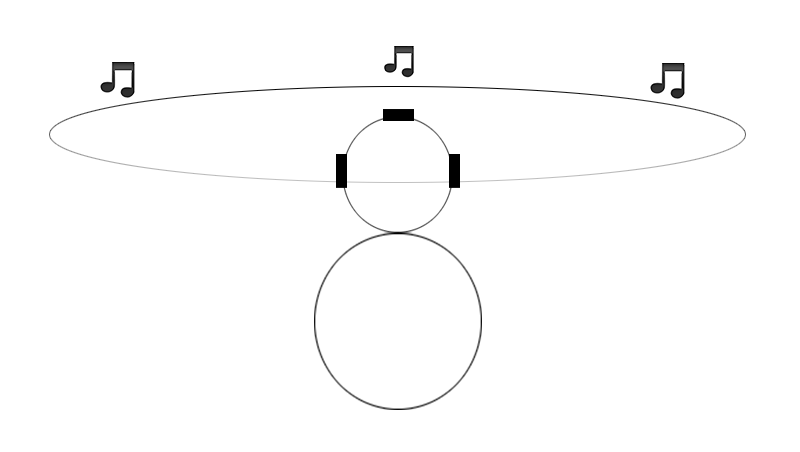
\includegraphics[width=0.6\textwidth,height=\textheight,keepaspectratio]{./Figures/sounddesign.png}
		\rule{35em}{0.5pt}
	\caption[Soundscape Design]{Soundscape Design - Visualising how the circular auditory menu surrounds a person (viewed from the persons back)}
	\label{fig:sounddesign}
\end{figure}

\subsection{Soundscape design}
\label{sec:designsoundscape}
The initial soundscape design is generally inspired from the Brewster et. al system \cite{brewster_multimodaleyes-freeinteraction_2003} mentioned in section \ref{sec:auditorygesturebasedmenus}. Non-speech sound items (music tracks) are layed out in a horizontal circular way within 140 degrees in front of the user, see figure \ref{fig:sounddesign}. The number of music tracks are spatially positioned and are playing simultanously. The menu uses exocentric interaction - by turning the head towards a music track, it will move in the center of the users front audio space. 2 kinds of interaction designs were to be tested by users. The two designs can best be described by imagining a carousel turning, while different music concerts play around it. In the first design the user stands in the center of the carousel looking out and in the second the user stands on the edge of the carousel looking out. These two interaction modes are illustrated in figure \ref{fig:interactionmodes}.

\begin{figure}[t]
	\centering
		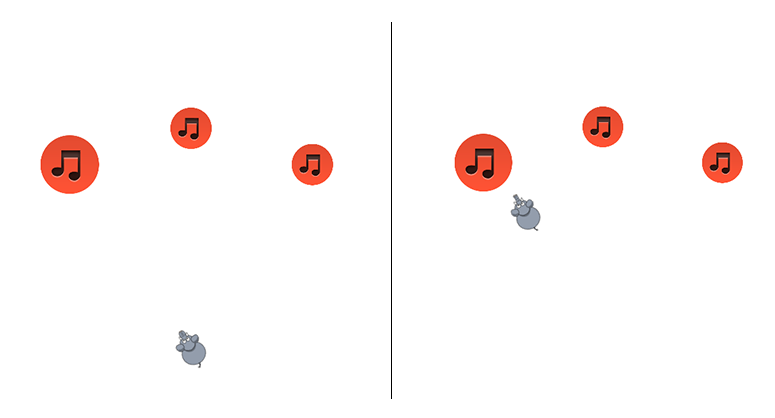
\includegraphics[width=0.9\textwidth,height=\textheight,keepaspectratio]{./Figures/interactionmodes.png}
		\rule{35em}{0.5pt}
	\caption[Interaction modes]{The system consists of two different interaction modes - with (to the right) and without (to the left) zoom feature. The user is illustrated by an elephant looking at the sound items.}
	\label{fig:interactionmodes}
\end{figure}

\textbf{1. User study}

The purpose of the first user study was to give qualitative feedback and specify appropriate parameters like max number of simultanous playing music tracks, the preferred degree for head rotation and the distance between the user and the music items for both interaction modes. Although not neccesary for the final design, we developed an envisionment prototype \cite{benyon_designing_2010} that visualised the actual soundscape design. This envisionment technique gave the users in the study a quicker and better understanding of the design. Figure \ref{fig:pilotstudy} shows a user testing the design and the envisionment prototype.

\begin{figure}[b]
	\centering
		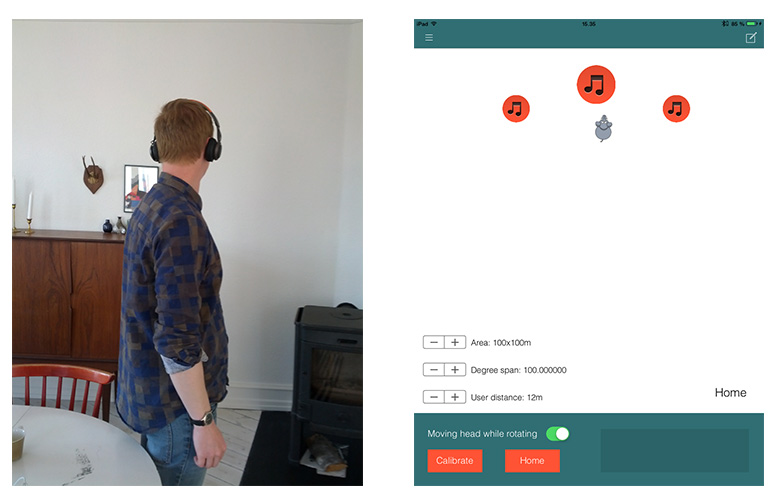
\includegraphics[width=0.9\textwidth,height=\textheight,keepaspectratio]{./Figures/pilotstudy.jpg}
		\rule{35em}{0.5pt}
	\caption[Pilot study]{Pilot study showing a user testing the design and the visual prototype.}
	\label{fig:pilotstudy}
\end{figure}

The music tracks used in the test were added by the users to make sure they knew the tracks. Both interaction modes were tested by starting laying out 3 sound items and then adding 1 item iteratively until the user found it too hard to recognize the music tracks. Distance and head rotation parameters were adjusted to match the user preferences every time sound items were added. The users preferred the interaction mode with zoom effect and they felt comfortable with 6-8 simultanous playing music tracks compaired to the other mode where \textgreater 4 simultanous music tracks were hard to segregate. Users preferred a smaller head rotation degree with the zoom effect of 80-100 degrees compaired to the other mode where 120-140 degrees were preferred. The feedback results are shown in table \ref{tab:pilotresults}.

\begin{table}[t] 
\scriptsize
\centering
\caption{Pilot study feedback} % title name of the table 
%\centering % centering table
\begin{tabular}{L{3cm}C{3cm}C{3cm}} \toprule
	 & Direction based & Direction based with zoom effect \\ \midrule
    Max number of music tracks   & 3-5 & 6-8 \\
    \\
    Preferred head rotation degree   & 120-140 & 80-100 \\ \bottomrule
\end{tabular}

\label{tab:pilotresults} 
\end{table}

There was a general agreement among the participants that the menu with zoom effect was preferred over the other.

\subsection{Navigation}
\label{sec:designnavigation}
The menu was designed with a 2 level exploring part that utilizes the soundscape design and a final level for playing the music track (simple playback). The idea is that the exploring starts by selecting an artist (HOME), then moving up a level to select a track from that artist (ALBUM) and then finally playing it (PLAYING TRACK). This menu hierachy design aimed to achieve the same rich exploration of music tracks that is provided by todays "stop-to-interact" music menus (described in section \ref{sec:alternativemusicuis}). 

A selection of a sound item is possible when it is in "focus" i.e. in the center of the user audio perspective. This focus range depended on the number of items and the chosen head rotation degree e.g. 120 degrees and 3 sound items gives a focus range of 40 degrees for each item. The menu hierachy (reversed) and examples on items that are in focus is illustrated in figure \ref{fig:navigation}.

\begin{figure}[b]
	\centering
		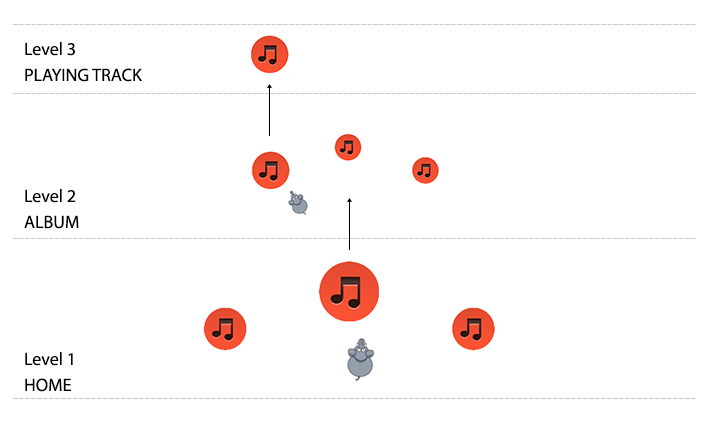
\includegraphics[width=0.8\textwidth,height=\textheight,keepaspectratio]{./Figures/navigation.png}
		\rule{35em}{0.5pt}
	\caption[Menu Hierachy]{The menu consists of 2 exploring levels and 1 level for playing track.}
	\label{fig:navigation}
\end{figure}

To navigate between levels simple head gestures were designed: A forward nod for going up one level, a backward nod for going back one level and a right sideways nod for activating the menu. Activating the menu would be the case where a music track is playing and the user wish to change track - it will take the user to the HOME level. When entering a level, audio feedback is given in form of speech recorded sounds telling what level the user is in e.g. "Home", "Album" and "Playing track". 

\textbf{2. User study}

The head gestures and the ability to navigate between menu levels were evaluated in a second user study. The same participants as in the first study and with the same chosen music tracks started by recording the 3 different gestures, 10 times for each gesture (10x3), to give us some training data. Then the participants simply tried to choose tracks by navigating between levels using the gestures. The system seemed to react to undesired gestures (false positives) when participants were rotating the head which affected the navigation experience negatively. Backward and sideways nods were removed and instead to go up one level or to activate the menu a simple push on a button on the headset were introduced. This helped in several ways - the user only needed to focus on 1 gesture which they also reported was the easiest gesture to conduct. For the systems point of view the nod is the most important gesture in that it is the actual selection of an item. We assume users most of the time to select the desired music track, and therefore going back a level would at least not be as neccesary as selecting i.e. we would not expect a lot of button push activity. Same theory goes for activating, this will be a 1 time push for every time the user wishes to change track. 

\textbf{3. User study}
We did a final small user study to test the nod gesture recognizers accuracy. A test user was asked to do 100 head gestures over time where every second gesture should be a nod and in between it should be anything else than a nod. By using classifier performance techniques \cite{fawcett_introduction_2006} we observed and noted down every gesture and labeled it using the confusion matrix, shown in figure \ref{tab:gestureconfusionmatrix}.

\begin{table}[h] 
\scriptsize
\centering
\caption{Nod gesture confusion matrix} % title name of the table 
%\centering % centering table
\begin{tabular}{C{4cm}C{4cm}C{4cm}}
	\hline
	 & Nod recognized by system & Nod NOT recognized by system\\ \midrule
	User did perform a nod & True positive & False positive \\
	 &  &  \\
	User did NOT perform a nod & False negative & True negative \\ \bottomrule
\end{tabular}
\label{tab:gestureconfusionmatrix} 
\end{table}

To get the accuracy we used the following equation:\\

$Accuracy = \dfrac{\sum{}True \: positive + \sum{}True \: negative}{\sum{}Total \: events}$\\

Table \ref{tab:gestureregistrations} shows the results. We end up with an accuracy of 92\%. Decreasing the number of gestures had the desired effect as no false positives were registered.

\begin{table}[h] 
\scriptsize
\centering
\caption{Nod gesture registrations} % title name of the table 
%\centering % centering table
\begin{tabular}{|C{3cm}|C{3cm}|C{3cm}|C{3cm}|}
	\hline
	True positive & False positive & True negative & False negative \\ \hline
	42 & 0 & 50 & 8 \\ \hline
\end{tabular}
\label{tab:gestureregistrations} 
\end{table}














% OLD - Use some parts here and move some to introduction method section


%A small accuracy test were conducted for nod selections by observing a user and the system response registering true postitives (nod performed and detected), true negatives (nod performed but not detected) and false positives (nod detected but not performed). The participant simply performed nods while turning the head in different directions in between and every event, whether it was a performed nod or a detected nod by the system, were noted down. Table \ref{tab:accuracytest} shows the results of 200 registered events - 100 from two different users.



%163 of 200 events were executed correctly so we end up with an accuracy of $\sim$ 82\%. Decreasing the number of gestures had the desired effect and the false positives were reduced to only 2 detections during the 200 events.


% Positive = Gesture recognized
% Negative = No gesture recognized


%The design is based on the following parameters: 

%\begin{itemize}
%\item Simultanous sounds (music tracks) spatially positioned
%\item Horizontal circular menu layout with music tracks as menu items
%\item Non-speech sound items in form of music tracks
%\item Simple speech sound feedback indicating menu level
%\end{itemize}

%- Music, strength of recognizing artist/track through listening vs seeing the text on a screen
%- Horizontal argument
%- Two menu interaction modes, distance/
%- Selective attention task
%- Simultanous sounds, exploring, cocktail party effect argument
%- Experimental design, sounds perceived, zoom effect, user should detect sound direction (which track)

% Horiontal alignment

% Circular

% non-speech sound

% selective-attention

% exocentric

% Head gestures, nod=yes


% From wiki:
% - the reasons behind a design decision,
% - the justification for it,
% - the other alternatives considered,
% - the trade offs evaluated, and
% - the argumentation that led to the decision.









